\section{Guidance Analysis and Visualization}
\label{sec:guidance-analysis}

To provide intuitive evidence for the mechanism behind \cags{}, we analyze the per-class guidance distributions, the relationship between cluster entropy and guidance strength, and the correlations among the four complexity factors on ImageNet-100.

\Cref{fig:guidance-analysis} presents three complementary views. Panel~(a) shows the distribution of per-class guidance scales ($\lambda$) under five different weight configurations. The entropy-only configuration produces the widest spread ($\sigma = 0.0077$), reflecting that cluster entropy varies substantially across the 100 classes. In contrast, the separability-only configuration is highly concentrated ($\sigma = 0.0057$) with most classes clustered near the minimum, confirming that inter-class separability produces near-constant guidance---as noted in the factor ablation (Section~\ref{sec:factor-ablation}). The full multi-factor \cags{} metric ($\sigma = 0.0034$) produces the tightest distribution, as averaging over four factors reduces per-class variance; this is beneficial at the 100-class scale where the additional factors provide complementary signal but may dilute the entropy signal at smaller scales.

Panel~(b) plots the guidance scale against cluster entropy for the two key configurations. The entropy-only guidance (coral) shows a clear monotonic relationship with entropy, assigning higher $\lambda$ to high-entropy classes. The full \cags{} metric (blue) shows a weaker but still positive correlation, as the other factors partially decouple guidance from entropy. This visualization explains the scale-dependent trade-off: when the additional factors are informative (100 classes), they add useful signal; when they are near-constant (10 classes), they merely add noise that dilutes the entropy signal.

Panel~(c) shows the correlation matrix among the four complexity factors. Notably, all pairwise correlations are weak ($|r| < 0.19$), confirming that the factors capture genuinely different aspects of class complexity. The near-zero correlation between entropy and mode count ($r = -0.03$) is particularly informative: although both relate to intra-class structure, entropy captures the \emph{balance} of cluster sizes while mode count captures the \emph{number} of clusters. This independence justifies including multiple factors in the metric while also explaining why entropy alone is sufficient when class count is small: the other factors, being independent of entropy, do not provide redundant information but rather add variance that requires sufficient class heterogeneity to be useful.

\begin{figure}[t]
\centering
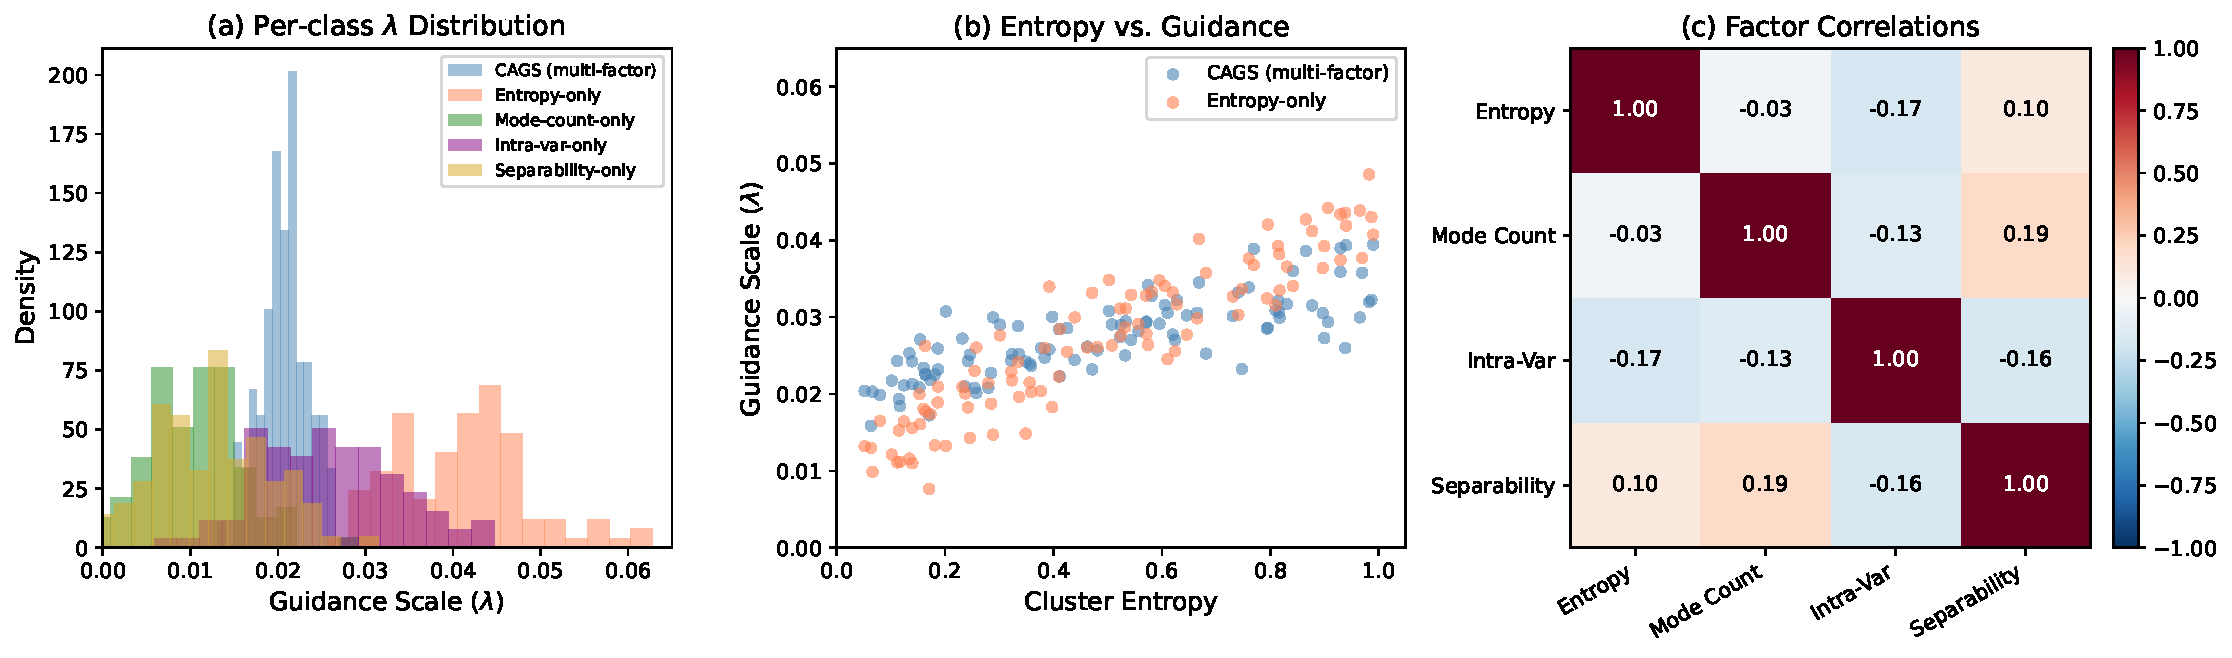
\includegraphics[width=\linewidth]{figures/guidance_analysis.pdf}
\caption{Guidance analysis on ImageNet-100. (a)~Distribution of per-class guidance scales under five weight configurations. Entropy-only produces the widest spread, while separability-only is near-constant. (b)~Cluster entropy vs.\ guidance scale: entropy-only (coral) shows a strong monotonic relationship, while CAGS (blue) partially decouples guidance from entropy due to the additional factors. (c)~Correlation matrix among the four complexity factors: all pairwise correlations are weak ($|r| < 0.19$), confirming they capture independent aspects of class complexity.}
\label{fig:guidance-analysis}
\end{figure}
